\section{Our process}\label{sprint1:ourprocess}
This semester our process has been inspired by the \texttt{Essence} process taught in the Software Innovation course.
We have previously been working with a ScrumBut approach, but decided that we wanted to try to improve our process by taking inspiration from a different process.\\
However, we have chosen to keep sprints, stand-up meetings and retrospective meetings from Scrum as these can complement Essence \cite{Essence}.
To make the report fit this format, it has been split into five sprints that fit the length of the semester, with each sprint lasting three weeks, except for the final sprint, sprint 5, which will only last two weeks due to time constraints.
The main aspect of Essence we drew inspiration from was the team organization.

\subsection{Team organization in Essence}
\label{sec:team-organization}
Within the team organization in Essence, roles are used to create heterogeneity in teams to ensure diverse points of view and to ensure cohesion despite diversity.
The focus of these roles is to increase learning with personal interaction by sharing insights and experiences.
The roles also try to ensure that the team understands the problem domain, and that it sees the potential solutions in the technology domain.
\\\\
The roles are persistent as a rule of thumb, meaning that a member will have the same role for the duration of the project.
The roles in Essence are compatible with agile software development, making it possible to combine Essence with other processes like Scrum.
\\\\
There are four roles in Essence:
\begin{itemize}
    \item Child
    \item Responder
    \item Challenger
    \item Anchor
\end{itemize}
The \textit{Child} can ask any questions and make propositions that are in opposition to previous decisions.
The rest of the team is not allowed to criticize the \textit{Child}, but they are however allowed to ignore their suggestions.
The \textit{Child} is one of the main sources of ideas and other perspectives on the project.
\\\\
\textit{Responders} are the developers in the team, and are usually the majority.
\textit{Responders} work closely together with the \textit{Challenger}, so that the most important features are developed first.
\\\\
\textit{Challenger} is the customer or customer representative.
The challenger can be compared to the \textit{Product Owner} in Scrum.
This role formulates and explains the challenge, which in Essence is the problem we are working on within the problem domain, prioritizes features and accepts the solutions.
There can be more than one \text{Challenger}, but if there are they must agree on the product vision.
\\\\
The \textit{Anchor} is the one responsible for leading evaluations, but does not decide the consequences.
If necessary, the \textit{Anchor} can intervene and remove threats to the team's ability to develop ambitious responses.
A potential threat could be something that results in productivity issues.

\subsection{Roles in practice}
We have divided the roles described in \autoref{sec:team-organization} between the members of the group.
One member has the \textit{Challenger} role, meaning that they are accountable for prioritizing the tasks in the backlog.
The process of prioritizing tasks is further described in the following section.
Another member has the \textit{Anchor} role, and is responsible for changes to the process as well as in charge of leading the stand up meetings, retrospectives and evaluations of the process.
The rest of the group functions as \textit{Responders}, which is the role for the developers of the project.
The \textit{Child} role fluctuates between members of the group.
Everyone can add suggestions to improve an idea and give other perspectives on the project. \\
The challenger and anchor will also work as developers during the duration of the project.

\subsection{Prioritizing tasks}
To keep track of what needs to be done, a shared backlog is saved on Jira which is a project management tool.
An example of the backlog can be seen on \autoref{fig:to-do-board}.
The leftmost column is the \textit{Suggested} column.
Everyone can make suggestions for tasks that they find useful for the project.
After each stand-up meeting, the challenger will present new suggestions that seem relevant to work on in the near future.
This presentation will include the definition of done (DoD), and all members of the group will then vote on how valuable it is for the project and how time-consuming it is expected to be.
The priority of a task is then calculated as $reward - time$, which is an arbitrary number to indicate how important it is.
\\\\
The challenger then chooses the most important tasks from the \textit{Discussed} column, often based on the priority, as \textit{Chosen for Development}.
Responders then have the opportunity to take tasks from this column and move it to the next column \textit{In progress} when they start working on it.
When the task has been completed, reviewed and merged into the develop branch, it is automatically moved to the column \textit{Done}.
\begin{figure}[H]
    \centering
    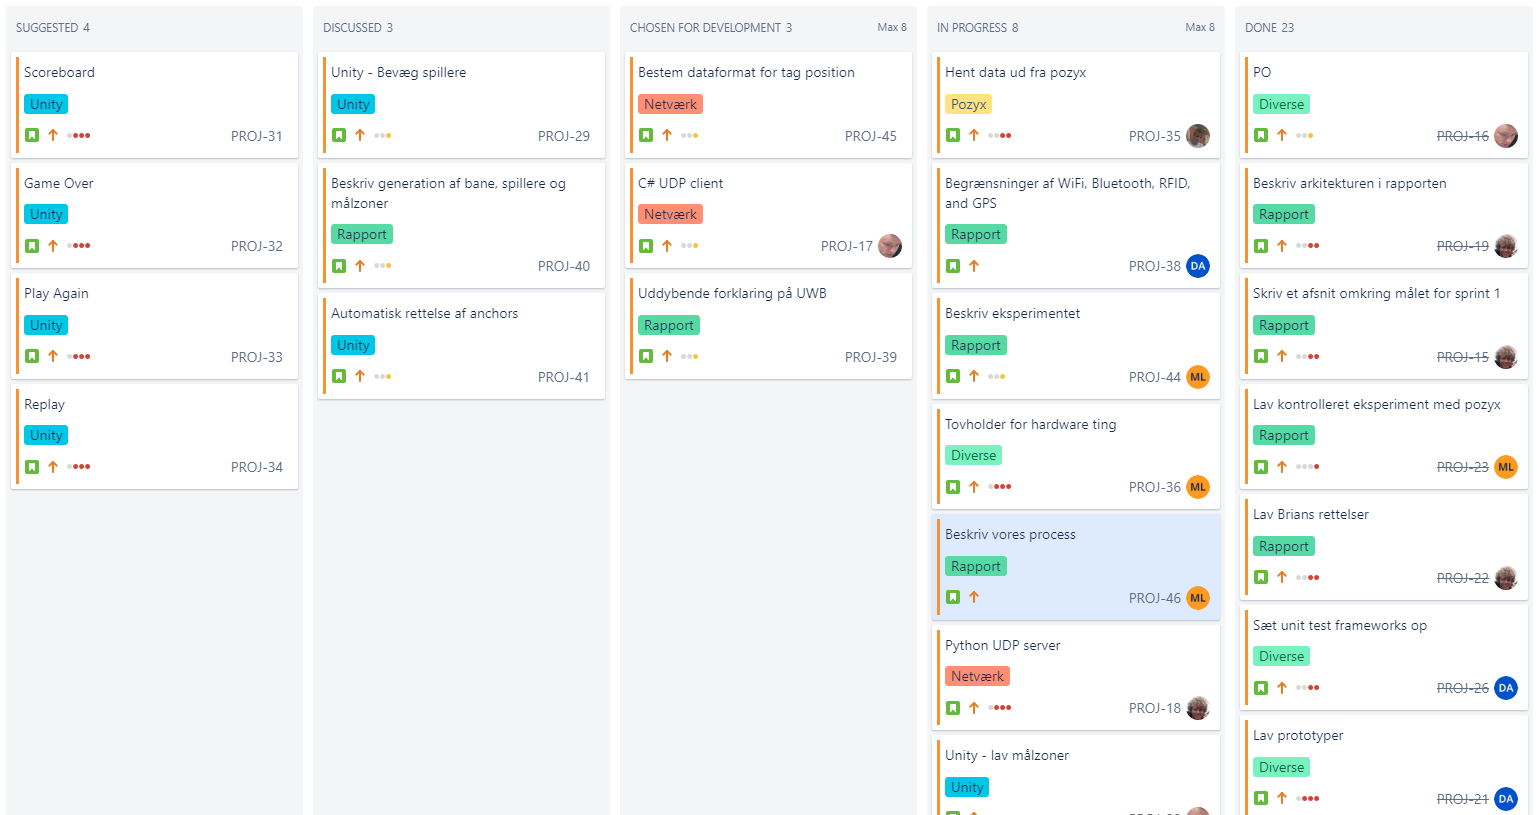
\includegraphics[width=\linewidth]{kanban.PNG}
    \caption{The board for tasks.}
    \label{fig:to-do-board}
\end{figure}

\subsection{Pair reviews}
Everything undergoes a formal review before it is added to the project in order to ensure quality.
This involves ensuring that the code is functional, that it implements the DoD, is readable and makes sense, as well as is accompanied by tests for parts of the system that might need it.
For report tasks, two reviewers are assigned to review and approve it before it can be merged.
For coding tasks, two people are likewise assigned to review it, but the review has to be done as a pair, meaning that they have to physically sit together and go through the code on a shared screen.
These pair reviews are a good way to share knowledge about the implementation through the group, as people have to understand it to be able to discuss it.
During previous semesters people have reviewed the code separately, which led to fewer comments as the code was not discussed between reviewers.